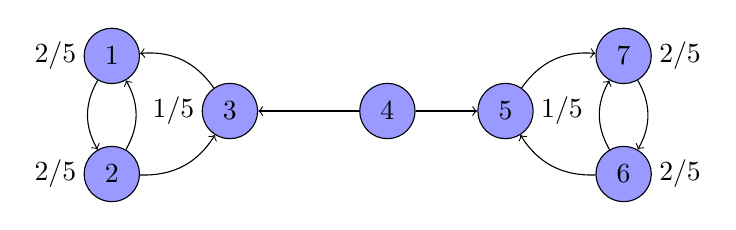
\begin{tikzpicture}
\tikzstyle{every node}=[draw,circle,fill=blue!40!white,minimum size=20pt,
inner sep=0pt]

\draw (-1.5,0)  node (1) [label=left:$2/5$] {1};
\draw (-1.5 ,-1.5)  node (2) [label=left:$2/5$] {2};
\draw (0,-0.7)  node (3) [label=left:$1/5$] {3};
\draw [->] (1) to  [bend right] (2);
\draw [->] (2)to  [bend right](1);
\draw [->] (3)to  [bend right](1);
\draw [->] (2)to  [bend right](3);
\draw (2,-0.7)  node (4) [label=left:$$] {4};
\draw [->] (4)to (3);
\draw (3.5,-0.7)  node (5) [label=right:$1/5$] {5};
\draw [->] (4)to (5);
\draw (5,0)  node (7) [label=right:$2/5$] {7};
\draw (5 ,-1.5)  node (6) [label=right:$2/5$] {6};

\draw [->] (7) to  [bend left] (6);
\draw [->] (6)to  [bend left](7);
\draw [->] (5)to  [bend left](7);
\draw [->] (6)to  [bend left](5);
\end{tikzpicture}